\documentclass{note}
\usepackage[cpp,table]{mypackage}
\usepackage{footnote}
\makesavenoteenv{tabular}

\def\ojoin{\setbox0=\hbox{$\bowtie$}%
  \rule[-.02ex]{.25em}{.4pt}\llap{\rule[\ht0]{.25em}{.4pt}}}
\def\leftouterjoin{\mathbin{\ojoin\mkern-5.8mu\bowtie}}
\def\rightouterjoin{\mathbin{\bowtie\mkern-5.8mu\ojoin}}
\def\fullouterjoin{\mathbin{\ojoin\mkern-5.8mu\bowtie\mkern-5.8mu\ojoin}}

\renewcommand{\thefootnote}{\fnsymbol{footnote}}
\lstset{language=sql}

\title{数据库系统原理笔记}
\author{陈鸿峥}
\date{{\builddatemonth\today}\protect\footnote{\text{Build \builddate\today}}} % protect!

\begin{document}

\maketitle
\renewcommand{\thefootnote}{\arabic{footnote}}
\setcounter{footnote}{0}

\setcounter{tocdepth}{2}%设置深度
\tableofcontents

\bigskip\bigskip

% !TEX root = main.tex

\section{计算机系统概述}
\subsection{计算模型}
\begin{itemize}
	\item 图灵机(1936)
	\item 冯诺依曼体系结构(1945)\footnote{非冯诺依曼体系结构:并行计算、量子计算、生物计算} --- 存储程序原理(\textbf{运算器}为中心)\\
	计算机采用\textbf{二进制}表示机器指令和数据,按照程序指令\textbf{顺序}执行
\begin{center}
\begin{tikzcd}
& & \text{存储器}\arrow{d} & & \\
\quad\arrow{r} & \text{输入设备}\arrow{r} & \text{运算器}\arrow{r}\arrow{d}\arrow{u} & \text{输出设备}\arrow{r} & \quad\\
& & \text{控制器}\arrow{u}\arrow{lu}\arrow{ru}\arrow[bend left]{uu} & &
\end{tikzcd}
\end{center}
而现在由于计算不是瓶颈,存储访问成为了瓶颈,故现代微机以\textbf{存储器}为中心
\begin{center}
\begin{tikzcd}
& & \text{运算器}\arrow{d} & & \\
\quad\arrow{r} & \text{输入设备}\arrow{r} & \text{存储器}\arrow{r}\arrow{d}\arrow{u} & \text{输出设备}\arrow{r} & \quad\\
& & \text{控制器}\arrow{u}\arrow{lu}\arrow{ru}\arrow[bend left]{uu} & &
\end{tikzcd}
\end{center}
\end{itemize}
[运算器、控制器](CPU)、存储器为计算机的核心,合称主机;外围设备,简称外设,指除主机外的其他设备,包括IO设备、外存等

计算机中的信息仍用二进制表示的原因:由物理器件性能决定
\begin{itemize}
	\item 二进制只有两种状态,容易找到具有2个稳定状态并且状态转换容易控制的物理器件(数字电路)
	\item 二进制编码运算规则简单
	\item 二进制的0、1与二值逻辑一致,容易实现逻辑运算
\end{itemize}
% There are two reasons computers use the binary system:
% 1.Two clearly distinct states that provide a safety range for reliability.
% 2.Least amount of necessary circuitry, which results in the least amount of space, energy consumption, and cost.

\subsection{计算机的发展历程}
按发展历程可分为:电子管、晶体管、集成电路、(超)大规模集成电路四代计算机
\par重大历史事件如下
\begin{center}
\begin{tabular}{|c|c|c|c|}
\hline
% 年份 & 姓名 & 事件 & 备注 \\
1904 & 弗莱明(Fleming) & 二极管 & \\\hline
1907 & 德福雷斯特(De Forest) & 三极管 & \\\hline
1938 & 香农(Shannon) & 布尔代数与二值电子器件(继电器) & 奠定数字电路基石 \\\hline
1946 & & 第一台通用计算机ENIAC & 十进制 \\\hline
1947 & \begin{tabular}{c}布莱顿(Brattain)\\
巴丁(Bardeen)\end{tabular} & 点接触晶体管 & \\\hline
1949 & 肖克利(Shockley) & 结型晶体管(1949) & 1956诺贝尔奖\\\hline
1950 & & 二进制和存储程序EDVAC & 实现冯诺依曼设想(组合进步) \\\hline
1958 & Jack Kilby & 集成电路 & 2000诺贝尔奖 \\\hline
1965 & Moore & 摩尔定律 & \begin{tabular}{c}
在价格不变的情况下,每18个月芯片上\\
晶体管数目翻倍,性能也提升一倍
\end{tabular}\\\hline
1971 & Intel & 第一款微处理器4004 & 10$\mu$m\\\hline
\end{tabular}
\end{center}

\subsubsection{单处理器(1971-2002)}
性能提升主要手段
\begin{itemize}
	\item 提升工作主频:KHz增长至GHz(生产工艺进步,流水线级数增加)
	\item 指令级并行(ILP)
\end{itemize}
\begin{proposition}[安迪-比尔定律]
Andy gives, Bill takes away. 安迪是原Intel CEO,比尔是原微软CEO,硬件厂商靠软件开发商用光自己提供的硬件资源得以生存
\end{proposition}
但遇到频率墙和功耗墙
\[\text{功耗(power)}\propto 1/2\times\text{CMOS电容}\times\text{电压}^2\times\text{转换(01)频率}\]
\par
2004年,Intel放弃4GHz Pentium4芯片开发,因无法解决散热问题,通过加快主频提升处理器性能的路走到尽头

\subsubsection{多核处理器(2005-)}
采用多核处理器不过是将硬件的问题丢到软件\footnote{“向多核的转变并不是因为我们在软件或体系结构技术上取得了中大突破而带来的。相反,这种转变是当单处理器体系结构发展遇到了难以克服的巨大障碍时,我们被迫作出的一种选择。”---Kurt Keutzer (UCB), \emph{The Landscape of Parallel Computing Research: A View from Berkeley}}
\begin{theorem}[阿姆达尔(Amdahl)定律]
\label{thm:amdahl}
\[\text{改进后的执行时间}=\text{受改进影响部分的执行时间}/\text{改进提高的倍数}+\text{不受影响的执行时间}\]
\[S_A=\frac{1}{s+(1-s)/N},\]
\end{theorem}
对计算机系统的某个部分采用并行优化措施后所获得的计算机性能的提高是有上限的,上限由串行部分所占的比例决定
\begin{theorem}[古斯塔夫森(Gustafson)定律]
\[S_G=(s'+p'\times N)/(s'+p')=N+(1-N)\times s',\]
其中,$s'$和$p'$为程序串行部分与可并行化部分在并行系统上执行的时间占总时间的比例,$N$为处理器数量,简便起见设总时间$s'+p'=1$
\end{theorem}
打破Amdahl定律\textbf{问题规模不变}的假设,任何足够大的任务都可以被有效地并行化,只要问题规模可扩展,并行所带来的加速比就可以扩展


\subsection{计算机系统的层次结构}
\begin{center}
\begin{tikzcd}
\text{高级语言层}\arrow{d}{}\\
\text{汇编语言层}\arrow{d}{}\\
\text{操作系统层}\arrow{d}{}\\
\text{指令系统层}\arrow{d}{}\\
\text{微体系结构层}\arrow{d}{}\\
\text{数字逻辑层}
\end{tikzcd}
\end{center}
程序编译运行过程:
\begin{center}
\begin{tikzcd}
\text{高级语言}\quad\arrow{r}{\text{预编译、编译}} & \quad\text{汇编语言}\arrow{r}{\text{汇编}} & \text{目标文件(二进制)}\arrow{r}{\text{链接}} & \text{可执行文件(二进制)}\arrow{d}{\text{加载}}\\
& & \text{电路上的电信号}\quad & \quad\text{二进制机器指令流(硬盘$\to$存储器)}\arrow[swap]{l}{\text{CPU取指译码}}
\end{tikzcd}
\end{center}
计算机内部工作过程:逐条执行加载到内存中的二进制机器指令流的过程

指令执行分为两个阶段,周期性重复性进行:
\begin{itemize}
	\item 取指阶段:CPU从内存中读取指令,程序计数器(PC)保存要被要被取出的\textbf{下一条}指令的地址,除非遇跳转指令,否则都加一个增量\footnote{程序计数器(Program Counter)是一个实际存在的寄存器吗? - Belleve的回答 - 知乎 \url{https://www.zhihu.com/question/22609253/answer/21965180} PC每次增加\textbf{一条指令的长度/寻址粒度},在MIPS中一条指令长4字节,寻址粒度1字节,故每次PC加4;而x86体系指令长度不定,每次增加量会变化}
	\item 执行阶段:对取出的指令译码后执行
\end{itemize}
软件系统可分为系统软件和应用软件

\subsection{计算机结构的八个想法}
\begin{enumerate}
	\item 摩尔(Moore)定律:集成电路资源每$18-24$个月翻倍
	\item 抽象(abstraction):简化设计
	\item 加速常用操作(Make common case fast):见定理\ref{thm:amdahl}
	\item 并行(parallelism)
	\item 流水线(pipelining)
	\item 预测(prediction)
	\item 内存等级制(hierarchy)
	\item 冗余实现可靠性(redundancy):检测故障及解决
\end{enumerate}

\subsection{基本指标}
表示计算机通信带宽时
\begin{center}
\begin{tabular}{ccccccc}\hline
KB(yte) & MB & GB & TB & PB & EB & ZB\\\hline
$10^3$ & $10^6$ & $10^9$ & $10^{12}$ & $10^{15}$ & $10^{18}$ & $10^{21}$\\\hline
\end{tabular}
\end{center}
表示计算机存储二进制时
\begin{center}
\begin{tabular}{ccccccc}\hline
KiB(yte) & MiB & GiB & TiB\\\hline
$2^{10}$ & $2^{20}$ & $2^{30}$ & $2^{40}$\\\hline
\end{tabular}
\end{center}
\begin{itemize}
	\item 位(bit/b):计算机处理、存储、传输信息的最小单位
	\item 字节(Byte/B) $1\text{ Byte}=8\text{ bit}$:现代计算机主存按字节编制,字节是最小可寻址单位
	\item 字(Word):表示被处理信息的单位,用来度量数据类型的宽度\footnote{字长是指CPU中\textbf{数据通路的宽度},等于CPU内部总线的宽度或运算器的位数或通用寄存器的宽度;字和字长的宽度可以一样,也可以不同,通常是字节的整数倍}
\end{itemize}
\par 一台32位的电脑,一个字等于4个字节,字长为32位;若字长为16位,则一个字等于2字节.
\par 4字节相当于8位16进制编码

\subsection{性能评价}
\label{subsec:performance}
CPU主频:对同一型号计算机,主频越高,完成指令一个执行步骤时间越短
\[\text{计算机的性能(Performance)}=1/\text{执行时间(Execution time)}\]
按照单位(量纲)进行换算即可
\[\begin{aligned}
\text{CPU执行时间(s)}&=\text{执行程序所需CPU时钟周期(cyc)}\times\text{时钟周期s/cyc)}\\
&=\text{指令数目(ins)}\times\text{CPI(cyc/ins)}\times\text{时钟周期(s/cyc)}
\end{aligned}\]
程序性能对执行事件的影响:
\begin{center}
\begin{tabular}{|c|c|c|c|}\hline
 & 指令数 & CPI & 时钟周期\\\hline
算法、编程语言、编译器 & $\times$ & $\times$ & \\\hline
指令集 & $\times$ & $\times$ & $\times$ \\\hline
计算机组成 & & $\times$ & $\times$ \\\hline
实现技术 & & & $\times$\\\hline
\end{tabular}
\end{center}
体系结构=指令集体系结构(功能定义与设计)+计算机组成(考虑用什么材料)\\
举例来说:
\begin{itemize}
	\item 指令集(ISA)考虑:是否提供乘法指令
	\item 组成(Organization)考虑:如何实现乘法指令(专门乘法器还是加法器+移位器)
	\item 实现技术(Technology)考虑:如何布线、用什么材料和工艺
\end{itemize}

% 带有处理器的设备一般称为智能化设备
% 完整的计算机系统应包括配套的硬件设备和软件系统
% !TEX root = main.tex

\section{SQL简介} % Chap 3
SQL即结构化查询语言(Structured Query Language, SQL)

\subsection{数据定义语言(DDL)}
数据类型
\begin{itemize}
	\item \verb'char(n)':固定长度字符串
	\item \verb'varchar(n)':可变长度字符串,用得最多
	\item \verb'int'
	\item \verb'smallint'
	\item \verb'numeric(p,d)':定点数,共$p$位(包括符号位),其中$d$位在小数点右侧
	\item \verb'real', \verb'double precision'
	\item \verb'float(n)':精度至少为$n$位的浮点数
\end{itemize}
\begin{lstlisting}[language=sql]
create table instructor (
	ID char(5),
	name varchar(20) not null,
	dept_name varchar(20),
	salary numeric(8,2) default 0,
	primary key (ID), -- integrity constraints
	foreign key (dept_name) references department);
\end{lstlisting}

\subsection{数据查询语言}
基本的形式如下所示
\begin{lstlisting}[language=sql]
select A1, A2, ..., An
from r1, r2, ..., rm
where P
\end{lstlisting}
其中$A_i$为属性(attribute)、$R_i$为一个关系(relation)/一个表、$P$是谓词(preicate),返回满足关系的数组。

\begin{itemize}
	\item 自然连接(natural join):将两个关系的各个元组进行连接,并且只考虑那些在两个关系模式中\textbf{都出现}的属性上取值相同的元组对(相当于取\textbf{交})
	\item 连接(join):用\verb'using'可以只考虑某一特定属性的连接
\end{itemize}
\begin{lstlisting}[language=sql]
select name, title
from (instructor natural join teachers) join course using (course_id);
-- only join two relations with the same course_id
\end{lstlisting}

字符串运算:模式匹配
\begin{itemize}
	\item \verb'upper(s)'、\verb'lower(s)'
	\item \verb'%':匹配任意字串
	\item \verb'_':匹配任意一个字符
	\item \verb'like':以这些字符串进行匹配
\end{itemize}

\begin{lstlisting}[language=sql]
select distinct dept_name
from instructor

select * -- all attributes
from instructor

select '437' as FOO

select ID, name, salary/12 as monthly_salary

select name
from instructor
where dept_name = 'Comp. Sci.' and salary > 80000

select *
from instructor, teaches -- Cartesian product

select distinct T.name
from instructor as T, instructor as S -- rename, Cartesian product
where T.salary > S.salary and S.dept_name = 'Comp. Sci.'
-- salary between 90000 and 100000

/**
percent ( % ). The % character matches any substring.
underscore ( _ ). The _ character matches any character.
**/
select name
from instructor
where name like '%dar%' matches any string containing "dar" as a substring

select distinct name
from instructor
order by name -- sorted

select *
from instructor
order by salary desc, name asc;

(select course_id from section where sem = 'Fall' and year = 2017)
union -- intersect, except
(select course_id from section where sem = 'Spring' and year = 2018)

select name
from instructor
where salary is null

-- aggregrate functions
-- arg, min, max, sum, count
select dept_name, avg (salary) as avg_salary
from instructor
where dept_name= 'Comp. Sci.'
group by dept_name;

select count (distinct ID)
from teaches
where semester = 'Spring' and year = 2018;

-- group constraints
-- find the average salary in each dept
select dept_name, avg(salary) as avg_salary
from instructor
group by dept_name -- can only be contained by select clause
having avg(salary) > 42000; -- effected after grouping
\end{lstlisting}

注意对于简单问题,通常没有必要用嵌套子查询,直接开几个关系即可
\begin{example}
对于下列两个关系表
\begin{itemize}
	\item Book(BID,title,AID,subject)
	\item Author(AID,first\_name,last\_name)
\end{itemize}
找出所有写了至少两种subject的作者的名字
\end{example}
\begin{analysis}
直接创建两个Book关系
\begin{lstlisting}
select a.last_name, a.first_name
from author a, book b1, book b2
where b1.aid = a.aid and b2.aid = a.aid and b1.subject != b2.subject
\end{lstlisting}
\end{analysis}

三值逻辑,添加了Unknown(其实就是T/F都恒成立的关系才会输出正常值)
\begin{center}
\begin{tabular}{|c|c|c|}\hline
AND & OR & NOT\\\hline
\begin{tabular}{l}
$T \land U = U$\\
$F \land U = F$\\
$U \land U = U$
\end{tabular} & 
\begin{tabular}{l}
$T \lor U = T$\\
$F \lor U = U$\\
$U \lor U = U$
\end{tabular} &
$\lnot U = U$\\\hline
\end{tabular}
\end{center}

SQL在谓词中使用\verb'null'测试空值,因而为找出\verb'instructor'关系中\verb'salary'为空值的所有教师,可写
\begin{lstlisting}
select name
from instructor
where salary is null
\end{lstlisting}

集合成员资格通过\verb'in'来判断,同时有\verb'some'和\verb'all'的关系测试,下面给出了一些嵌套子查询的例子。
\begin{lstlisting}
select name
from instructor
where salary > some (select salary
					from instructor
					where dept_name = 'Biology')

select S.ID, S.name
from student as S
where not exists ((select course_id
				from course
				where dept_name = 'Biology')
				except
				(select T.course_id
				from takes as T
				where S.ID = T.ID))

select T.course_id
from course as T
where 1 >= (select count(R.course_id)
			from section as R
			where T.course_id = R.course_id and R.year = 2009);
-- there is no unique in MySQL

with max_budget(value) as
	(select max(budget)
	from department)
select budget
from department, max_budget
where department.budget = max_budget.value;

select dept_name,
	(select count(*)
	from instructor
	where department.dept_name = instructor.dept_name)
	as num_instructors
from department; -- scalar subquery
\end{lstlisting}

数据库的修改操作如下
\begin{lstlisting}
delete from instructor
where dept_name = 'Finance';

insert into course(course_id, title)
	values ('CS-437','Database Systems');

update instructor
set salary = salary * 1.05
where salary < 70000;

update instructor
set salary = case
			when salary <= 1000 then salary * 1.05
			when salary <= 2000 then salary * 2.05
			else salary * 1.03
		end
\end{lstlisting}
% !TEX root = main.tex

\section{进阶SQL} % Chap 4
\subsection{内外连接}
\verb'on'条件可以提供比自然连接更为丰富的连接条件
\begin{lstlisting}
select *
from students join takes on student.ID = takes.ID; -- condition
\end{lstlisting}

直接使用\verb'natural join'可能导致元组丢失,比如有一些学生没有选修任何课程,则其在student关系中不会与takes关系中任何元组配对。
因此有\textbf{外连接}:
\begin{itemize}
	\item 左外连接(left outer join):只保留出现在左外连接运算之前(左边)关系中的元组,若右侧关系中没有对应属性则用null代替
	\item 右外连接(right outer join)
	\item 全外连接(full outer join):左外连接和右外连接的组合
\end{itemize}

从而可以很容易查询出“所有课程一门也没有选修的学生”:
\begin{lstlisting}
select ID
from student natural left outer join takes
where course_id is null;
\end{lstlisting}

为了将常规连接和外连接区分开,SQL中将常规连接称为内连接(inner join),默认的都是内连接。

\subsection{视图}
让用户看到整个逻辑模型显然是不合适的,出于安全考虑,可能需要向用户隐藏特定的数据。
本来通过select可以把需要的数据计算并存储下来,但一旦底层数据发生变化,查询的结果就不再匹配。
因此,为了解决这样的问题,SQL提供一种虚关系,称为视图(view),只有在使用的时候才会被计算。
\begin{lstlisting}
create view faculty as
select ID, name, dept_name
from instructor;
\end{lstlisting}
之后便可以直接使用\verb'from'语句访问视图。

\begin{definition}[物化视图(materialized view)]
如果用于定义视图的实际关系改变,视图也会跟着修改。
\end{definition}

由于视图并不是数据库底层的关系,故一般数据库不允许对视图关系进行修改。

\subsection{事务}
SQL标准规定当一条SQL语句被执行,就隐式开始了一个事务。
下列SQL语句之一会结束一个事务:
\begin{itemize}
	\item Commit work:将事务所做的更新在数据库中持久保存。
	在事务被提交后,一个新的事务自动开始。
	\item Rollback work:撤销该事务中所有SQL语句对数据库的更新,数据库将恢复到执行该事务的第一条语句之前的状态。
	如果遇断电,回滚会在下一次重启时自动执行。
\end{itemize}

\subsection{完整性约束}
单个关系上的约束
\begin{itemize}
	\item \verb'not null':跟在属性定义后面
	\item \verb'unique (A1,A2,...,Am)':声明$A_1,\ldots,A_m$构成一个候选码
	\item \verb'check(<predicate>)':关系中每个元组都必须满足该谓词,如\verb'check(budget>0)'
\end{itemize}

参照完整性/子集依赖:外码
\begin{lstlisting}
foreign key (dept_name) references department
	on delete cascade
	on update cascade
\end{lstlisting}
会级联(cascade)删除或更新。

\subsection{授权}
\verb'grant'授权,\verb'revoke'回收
\begin{itemize}
	\item \verb'select':允许用户修改关系中任意数组
	\item \verb'insert'
	\item \verb'delete'
\end{itemize}
用户名\verb'public'包括了当前所有用户和未来用户的权限。

\begin{lstlisting}
grant <authorization list>
on <relation name/view name>
to <user/user list>

grant update (budget) on department to Amit, Satoshi;
\end{lstlisting}

可以先创建角色(role)然后给用户授予角色。
% !TEX root = main.tex

\section{形式化关系查询语言} % Chap 6
\subsection{关系代数}
\begin{center}
\begin{tabular}{|c|c|c|}
\hline
选择 & $\sigma$ &
\begin{tabular}{l}
挑选出符合一定性质的元组\\
$\sigma_{\text{Sub="Phy"}\land\text{age}>30}(\text{teachers})$
\end{tabular}\\\hline
投影 & $\Pi$ & 
\begin{tabular}{l}
只选出对应属性\\
$\Pi_{\text{ID,name,salary}}(\text{teachers})$
\end{tabular}\\\hline
笛卡尔积 & $\times$ & 将两个关系整合(简单并置,需要进一步筛选)\\\hline
自然连接 & $r\Join s=\prod_{R\cup S}(\sigma_{r.A_1=s.A_1\land\cdots\land r.A_n=s.A_n})(r\times s)$ & \\\hline
$\theta$连接 & $r\Join_\theta s=\sigma_\theta(r\times s)$ & \\\hline
外连接 & $\leftouterjoin, \rightouterjoin, \fullouterjoin$ & \\\hline
并集 & $\cup$ & 数目应相同,属性可兼容\\\hline
交集 & $\cap$ & \\\hline
差集 & $-$ & \\\hline
赋值 & $\gets$ & \\\hline
重命名 & $\rho_x(E)$ & 给$E$的返回值赋名为$x$\\\hline
\end{tabular}
\end{center}

扩展的关系代数运算:
\begin{itemize}
	\item 广义投影:$\prod_{F_1,F_2,\ldots,F_n}(E)$,其中$F_i$中每一个都是涉及常量及$E$的模式中属性的算术表达式
	\item 聚类:$\mathcal{G}$,如count, min, max,考虑group by可以写成下列形式
	\[{}_{dept\_name}\mathcal{G}_{\textbf{average}(salary)}(instructor)\]
\end{itemize}

\begin{definition}[聚集运算]
聚集运算$\mathcal{G}$的通常形式如下:
\[{}_{G_1,G_2,\ldots,G_n}\mathcal{G}_{F_1(A_1),\ldots,F_n(A_n)}(E)\]
其中$E$是任意关系代数表达式,$G_1,\ldots,G_n$是用于分组的一系列属性;
每个$F_i$是一个聚集函数,每个$A_i$是一个属性名。
$E$结果中的元组将会以如下方式分为若干组:
\begin{itemize}
	\item 同组中所有元组在$G_1,\ldots,G_n$上的取值相同
	\item 不同组中的元组在$G_1.\ldots,G_n$上的取值不同
\end{itemize}
\end{definition}

\subsection{其他关系演算}
\subsubsection{元组关系演算}
元组关系演算是非过程化的查询语言(有点像声明式语言),它只描述所需信息,而不给出获得该信息的具体过程。
查询表达为
\[\{t\mid P(t)\}\]
即使谓词$P$为真的元组$t$的集合,$t[A]$表示元组$t$在属性$A$上的值,用$t\in r$表示元组$t$在关系$r$中。

如工资大于80000美元的所有教师的ID为(注意这里涉及到属性选择)
\[\{t\mid\exists s\in instructor(t[ID]=s[ID]\land s[salary]>80000\}\]

其实与命题逻辑类似
\[t\in\text{instructor}\land\exists s\in\text{department}(t[\text{dept\_name}]=s[\text{dept\_name}])\]
前者$t$为自由变量,后者$s$为受限变量。

元组关系演算可能产生一个无限的关系
\[\{t\mid\lnot(t\in instructor)\}\]
这样的元组有无限多个且不在数据库中,因此这样写是\textbf{不安全的}。

因此引入元组关系公式$P$的域的概念,如$\dom(t\in instructor\land t[salary]>80000)$是包括80000和出现在instructor中的所有值集合。
若表达式$\{t\in P(t)\}$结果所有值均来自$\dom(P)$,则说表达式$\{t\in P(t)\}$是安全的。

\subsubsection{域关系演算}
\[\{<x_1,x_2,\ldots,x_n>\mid P(x_1,x_2,\ldots,x_n)\}\]
其中$<x_1,\ldots,x_n>\in r$,每一个$x_i$为域变量,$r$为$n$个属性上的关系。

与元组关系演算最大的区别在于,域关系演算更加细粒度。
比如找出工资大于80000美元的所有教师的ID:
\[\{<i>\mid\exists n,d,s(<i,n,d,s>\in instructor\land s>80000)\}\]

同样有安全性问题,可类似定义。
% !TEX root = main.tex

\section{关系型数据库设计}
数据库设计的范式(normal form)
\begin{itemize}
	\item 第一范式:原子性,即所有元素都是不可分的单元
	\item 
\end{itemize}

\begin{definition}[函数依赖(functional dependency)]
设$R$为关系模式,$\alpha\subset R,\beta\subset R$,函数依赖$\alpha\to\beta$在$R$上满足,当且仅当对于任意合法的关系$r(R)$,任何两个关于$r$的数对$t_1$和$t_2$,如果满足属性$\alpha$,那么它们也满足属性$\beta$,即
\[t_1[\alpha]=t_2[\alpha]\implies t_1[\beta]=t_2[\beta]\]
实际上就是函数单射的概念。
\end{definition}
考虑下例$r(A,B)$的关系
\begin{center}
\begin{tabular}{|c|c|}\hline
A & B\\\hline
1 & 4\\\hline
1 & 5\\\hline
3 & 7\\\hline
\end{tabular}
\end{center}
关系$A\to B$不成立,但关系$B\to A$成立。

\begin{definition}[多值依赖(multivalued dependency)]
设$R$为关系模式,$\alpha\subset R,\beta\subset R$,多值依赖在$R$上满足$\alpha\twoheadrightarrow\beta$,
当且仅当对于所有数对$t_1$和$t_2$,使得$t_1[\alpha]=t_2[\alpha]$,都存在数对$t_3$和$t_4$使得
\[\begin{aligned}
\displaystyle t_{1}[\alpha ]&= t_{2}[\alpha ]=t_{3}[\alpha ]=t_{4}[\alpha ]\\
\displaystyle t_{3}[\beta ]&= t_{1}[\beta ]\\
\displaystyle t_{3}[R-\beta ]&= t_{2}[R-\beta ]\\
\displaystyle t_{4}[\beta ]&= t_{2}[\beta ]\\
\displaystyle t_{4}[R-\beta ]&= t_{1}[R-\beta ]
\end{aligned}\]
简而言之,设${\displaystyle (x,y,z)}$有对应着属性${\displaystyle \alpha ,}{\displaystyle \beta ,}{\displaystyle R-\alpha -\beta }$,则对于任意$R$中的元素${\displaystyle (a,b,c)}$和${\displaystyle (a,d,e)}$,都有${\displaystyle (a,b,e)}$和${\displaystyle (a,d,c)}$在$R$中
\end{definition}
% !TEX root = main.tex

\section{事务}
\begin{definition}[事务(transaction)]
构成单一逻辑工作单元的操作集合称为事务。
即使有故障,数据库系统也必须保证数据库的正确执行——要么执行整个事务,要么属于该事务的操作一个也不执行。
\end{definition}

事务具有以下的基本性质:
\begin{itemize}
	\item 原子性:要么执行完,要么不执行,不能执行到一半。
	\item 一致性:除了基本的数据完整性约束,还有更多的一致性约束。
	\item 隔离性:每个事务都察觉不到系统中有其他事务在并发执行,一定是完成一个再进行下一个。
	\item 持久性:一个事务成功完成对数据库的改变是永久的,即使出现系统故障。
\end{itemize}

事务的基本状态:
\begin{itemize}
	\item 活动的(active):初始状态
	\item 部分提交的(partially commited):最后一条语句执行后
	\item 失败的(failed):执行出错
	\item 中止的(aborted):事务回滚且数据库已恢复到事务开始执行前
	\item 提交的(commited):成功完成
\end{itemize}
\begin{figure}[H]
\centering
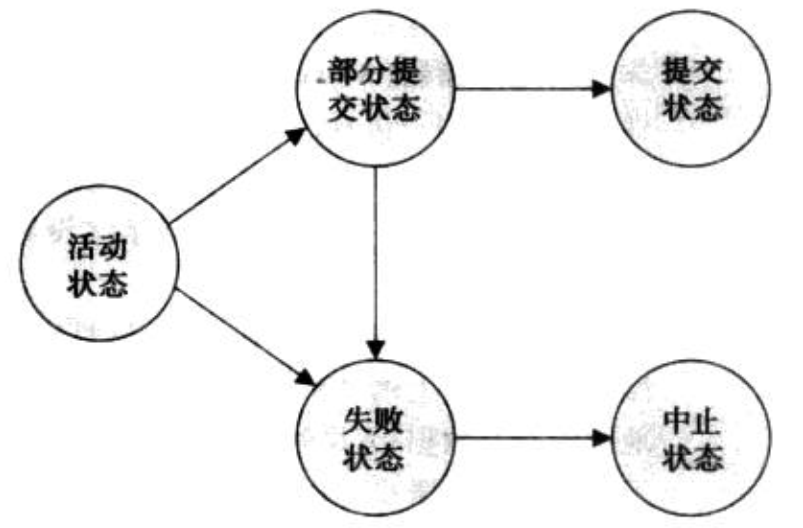
\includegraphics[width=0.5\linewidth]{transaction_state.png}
\end{figure}

\begin{definition}[冲突]
当$I$和$J$是不同事务在相同数据项上的操作,并且其中至少有一个是\verb'write'指令时,则称$I$与$J$是冲突的。
\end{definition}
\begin{definition}[冲突等价(conflict equivalent)]
如果调度$S$可以经过一系列非冲突指令交换转换为$S'$,则称$S$和$S'$是冲突等价的。
若$S'$为穿行调度,则$S$为冲突可串行化的(conflict serializable)。
\end{definition}

可以通过构造一个优先图(precedence graph)来判断是否冲突可串行化。
如果无环(用环检测算法),则冲突可串行化,可以通过拓扑排序得到串行化顺序。

\end{document}

% 1,2,3,4,6,7,8,10,11,14,15,16